%!TEX root = ../main.tex
\setcounter{chapter}{7}
\setcounter{section}{2}
\section{Design using Discrete Equivalents}
\vspace{-8pt} \hrule \hrule \hrule \hrule \hrule  \vspace{12pt}
Matlab Code
\begin{lstlisting}
clc;clear all; format compact; close all;
s=tf('s');
Dc = 10*(s/2+1)/(s/10+1)
Ts = 0.025;
Dz = c2d(Dc,Ts,'zoh');
[num,den]=tfdata(Dz);
Dz = tf(num,den,Ts,"Variable","z^-1")
figure(1)
step(Dc);
hold on;
step(Dz)
\end{lstlisting}
\url{https://github.com/tjdalsckd/ControlSystem_Lecture8/blob/main/matlab/ex8_2.m}\\
Result
\begin{lstlisting}
% Dc =
%   100 s + 200
%   -----------
%    2 s + 20
% Dz = 50 - 47.79 z^-1
%   ---------------
%   1 - 0.7788 z^-1 
% Sampling Time: 0.025 seconds
\end{lstlisting}
\newpage
\begin{figure}[h]
	\centering
	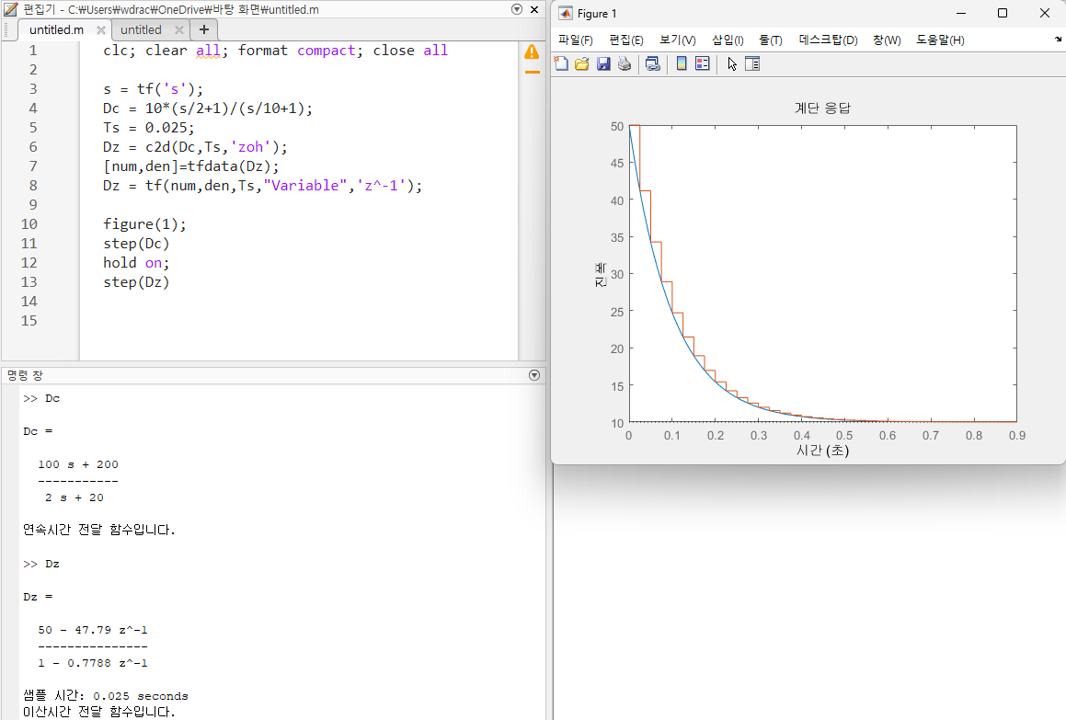
\includegraphics[width=20cm]{./FIG_Franklin/fig8-smc9.png}
\end{figure}